\section{Introduction}
\label{sec:introduction}

This work began from a surprising observation: even \emph{untrained}, randomly drawn embeddings appended to LLM inputs lift reasoning accuracy and reshape early decoding in several settings --- with no optimization at all. As LLMs scale, full fine-tuning is prohibitive, motivating parameter-efficient methods \citep{hu2022lora, houlsby2019adapter}. Among these, \textit{soft prompts} insert learnable continuous embeddings into the input and steer behavior through attention \citep{li2021prefix, lester2021power}; the paradigm is actively adopted for mathematical reasoning \citep{kang2025model, xu2025softcot, ye2025thinking, hao2024training, zhang2025memgen}. These methods diverge in injection position, training objective, and prompt form, and prior work attributes their gains to the \emph{learned content} of the optimized vectors. What every variant shares --- the act of injecting embeddings into the input --- has remained outside the analysis.

\begin{figure}[!t]
  \centering
  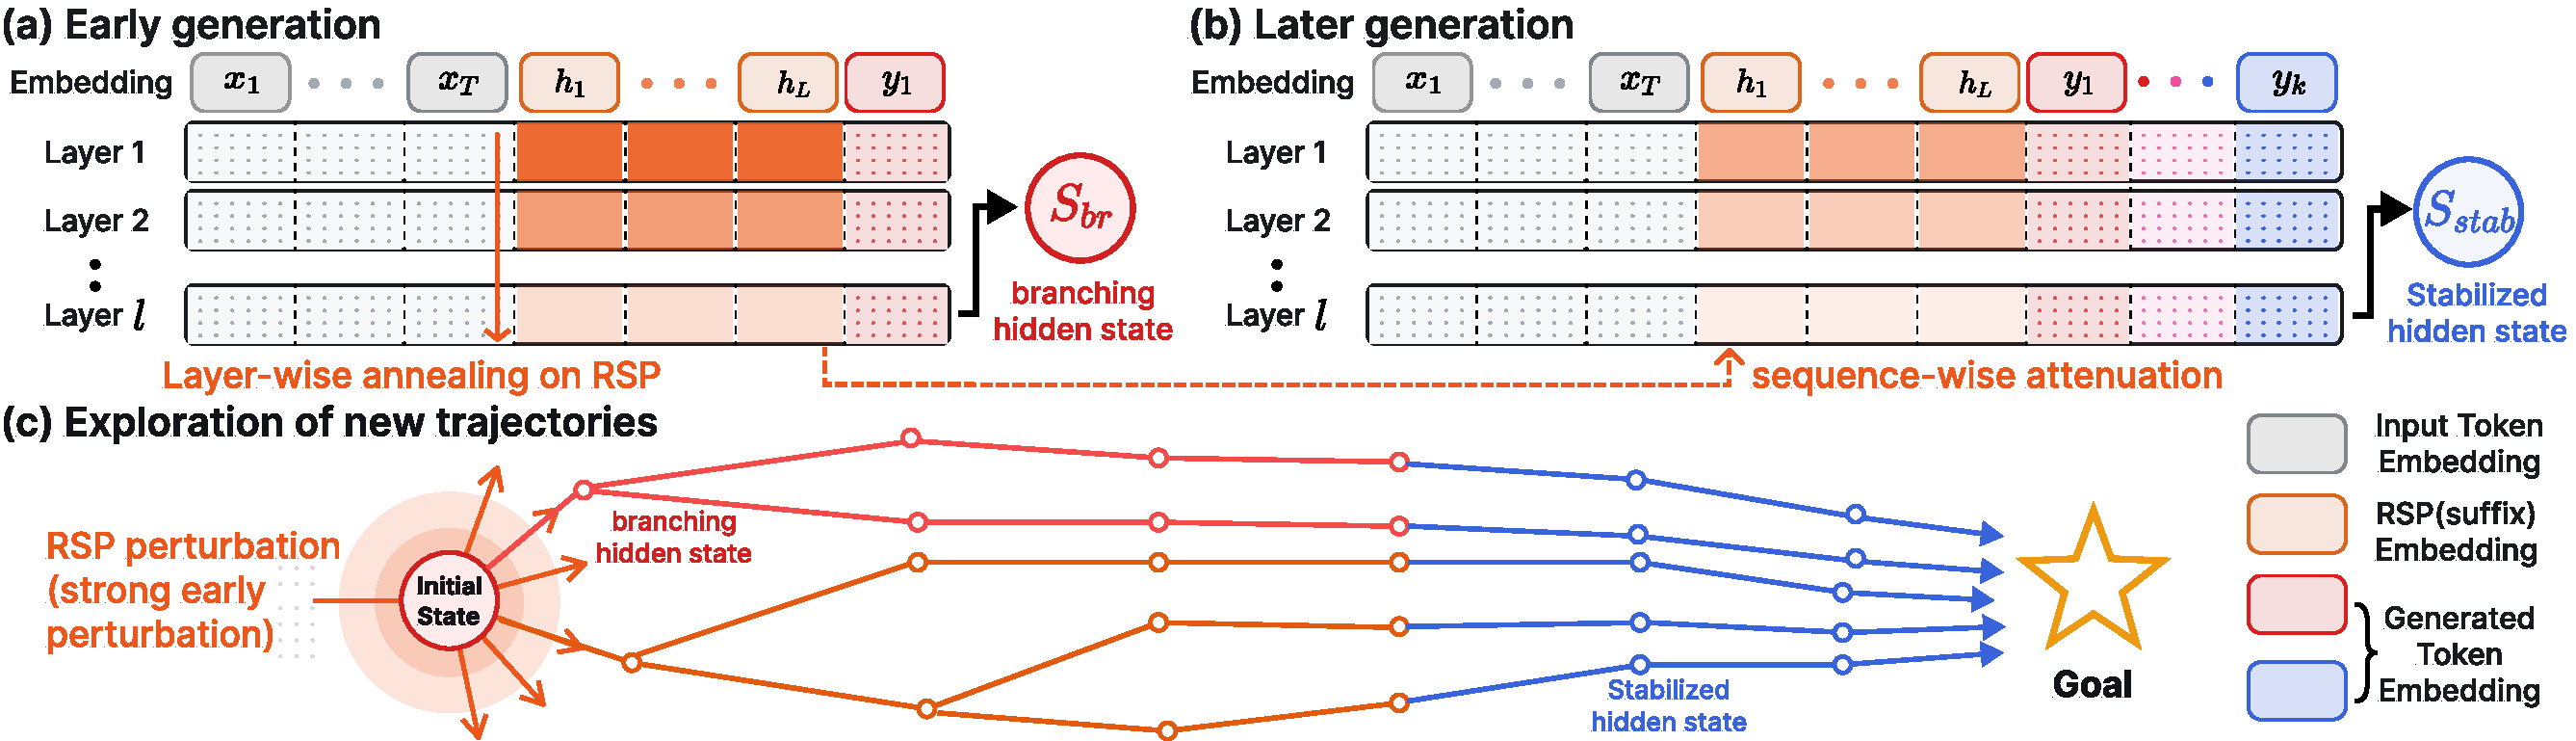
\includegraphics[width=\textwidth]{img/main/main.pdf}
  \caption{Conceptual overview of RSP-induced trajectory diversity. The hidden states shown are the final-layer outputs that drive the next-token distribution. (a) Early decoding: RSP perturbation reaches a \emph{branching state} (red; formalized in \S\ref{sec:rsp_definition}), whose top-$K$ differs from the no-RSP baseline and induces a diverse output distribution. (b) Later decoding: as the KV cache grows, the bound on RSP attention mass narrows (Theorem~\ref{thm:decay}); branching events become rare and the hidden state (blue) commits to the branch already opened. (c) Across rollouts, the trajectories opened by early RSP perturbation accumulate into independent paths.}
  \label{fig:main}
\end{figure}

To separate \emph{learned content} from the \emph{act of injection}, we use random soft prompts (RSPs) as a control --- continuous vectors drawn from an isotropic Gaussian fitted to the embedding table's mean and variance, with no learning. The control turns out to be non-neutral. Applying a chat template to a base model not fine-tuned for it degrades reasoning, yet appending RSPs recovers up to $+29$ pp on Qwen2.5-Math-1.5B; if simple noise were merely shaking the model, accuracy should have worsened instead. The injection itself, independent of any learned content, alters model behavior.

We analyze training-free Random Soft Prompts (RSPs) on LLM reasoning. With each rollout receiving an \emph{independent} draw, a single RSP injection \emph{branches} hidden states into diverse trajectories early on, which then \emph{stabilize} as decoding proceeds. Empirically, RSPs share the early-decoding entropy signature of optimized methods (LTPO, TTSV, SoftCoT) despite carrying no learned content; Pass@$N$ accumulates only under \emph{independent} resampling; and the same input-side diversity composes with DAPO \citep{yu2025dapo} training. Our contributions are: (i) RSP isolates the simplest form of soft prompt --- training-free and freshly resampled per rollout --- providing a unified lens for the structural effect of injection across variants that otherwise differ in training objective and prompt form, while still reaching accuracy comparable to optimized methods in several settings; (ii) a theoretical and empirical account of the mechanism (attention-mediated branch opening, isotropic directional coverage, KV-cache attenuation); and (iii) DAPO extension showing independent RSP resampling composes with rollout-diversity training.
